\chapter{\textsc{Introdution d'une correction numérique }}
\section{\textsc{L'effet du temps de conversion et les temps d'exécution}}

\par Lorsque le temps de conversion A/N, N/A et les temps d'exécution seront négligés, la période d'échantillonnage calculée ne sera pas éronnée.\\

   \section{\textsc{L'effet du temps de conversion et les temps d'exécution}}
   
   \par Le rôle du pôle $z=1$ du correcteur $C_1(z^{-1}$ est d'éliminner l'eereur de traînage. Celui du zéro $b_1$ est d'éliminer le rôle du pôle $z=b_1$ de $B_0G(z^{-1})$. Le rôle du pôle $z=-a_2$ est d'éliminer l'effet du zéro $z=-a_2$ de $B_0G(z^{-1})$. Enfin le rôle du zéro $a$ est d'éliminer l'effet du pôle $z=1$.\\[0.5 cm]
   \par a doit être comprise entre 0 et 1 pour des raisons de stabilité.
   
   \section{\textsc{Visualisation de $s(t)$ pour différentes valeurs de $a$}}
   
   	\begin{center}
	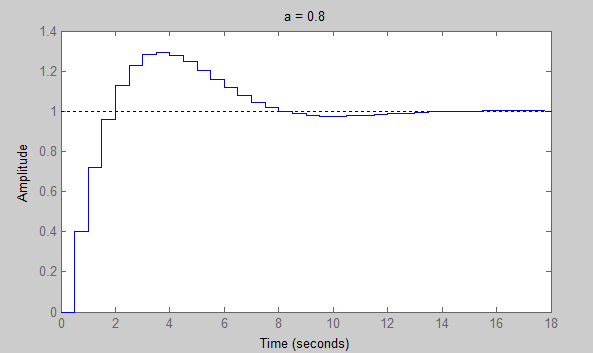
\includegraphics[scale=0.5]{a8.png}
	\captionof{figure}{\textit{Tracé de la sortie  $ s(t) $ pour $a=0.8$. \\}}
	\label{fig13} 
	\end{center}
	
		\begin{center}
	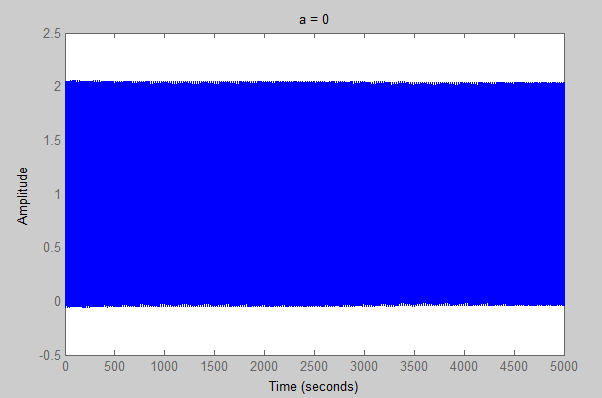
\includegraphics[scale=0.5]{a0.png}
	\captionof{figure}{\textit{Tracé de la sortie  $ s(t) $ pour $a=0$. \\}}
	\label{fig14} 
	\end{center}
	
		\begin{center}
	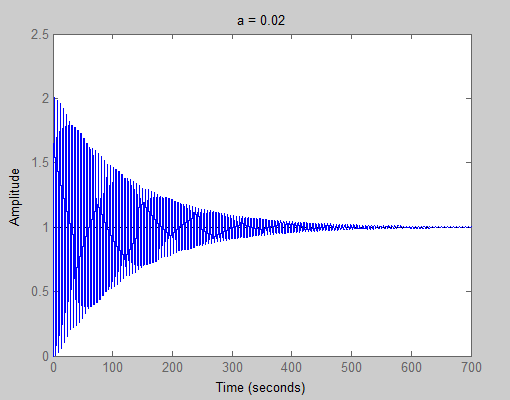
\includegraphics[scale=0.5]{a2.png}
	\captionof{figure}{\textit{Tracé de la sortie  $ s(t) $ pour $a=0.02$. \\}}
	\label{fig15} 
	\end{center}
 	
 		\par Il est clair qu'on choisira $a=0.8$ car c'est la seule valeur ou le système converge.
 		
 \section{\textsc{Stabilité du système en boucle ouverte avec correcteur par les lieux des racines pour différentes valeurs de $a$}}
 
 		\begin{center}
	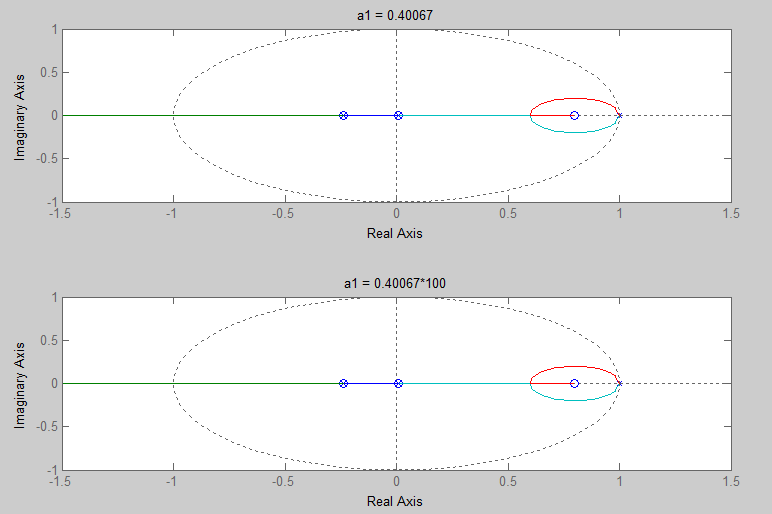
\includegraphics[scale=0.5]{rl3.png}
	\captionof{figure}{\textit{Rlocus pour $a1=0.4007$ et pour $a1=4.007$ . \\}}
	\label{fig17} 
	\end{center}
		
	\par Même pour une valeur de $a_1$ dix fois plus grande, la stabilité du système n'est pas affectée. Tous les pôles sont à l'intérieur du disque unité.
  	
\chapter*{\textsc{Conclusion}}
\addcontentsline{toc}{chapter}{\textsc{Conclusion}}
  
  \par A défaut de temps nous n'avons pas pu finir les parties restantes de cette séance de TP. On tient à s'excuser auprès de M Gouaisbaut et de M Fergani.